\documentclass[10pt,table, xcolor=pdflatex]{beamer}
\usepackage{newcent}
\usepackage[utf8]{inputenc}
\usepackage[czech]{babel}
\usepackage{hyperref}
\usepackage{textpos}
\usepackage{multicol}
\usepackage{tikz}
\usepackage{fancyvrb}
\usepackage{color}
\usepackage{subfig}
\usepackage{geometry}
\usepackage{graphicx}
\usepackage{epstopdf}

\usepackage{todonotes}
\usepackage{listings}

\makeatletter
\g@addto@macro{\UrlBreaks}{\UrlOrds}
\makeatother

\newcommand{\emp}{\lstinline[language={[LaTeX]TeX}, basicstyle=\tt\color{fitdark}]}

\lstdefinelanguage{XML}
{
  basicstyle=\ttfamily\footnotesize,
  morestring=[b]",
  moredelim=[s][\color{red!70!black}]{<}{\ },
  moredelim=[s][\color{red!70!black}]{</}{>},
  moredelim=[l][\color{red!70!black}]{/>},
  moredelim=[l][\color{red!70!black}]{>},
  morecomment=[s]{<?}{?>},
  morecomment=[s]{<!--}{-->},
  commentstyle=\color{black},
  stringstyle=\color{brown!80!black},
  identifierstyle=\color{violet}
}
\lstset{language=Java,
  showspaces=false,
  showtabs=false,
  breaklines=true,
  showstringspaces=false,
  breakatwhitespace=true,
  commentstyle=\color{green!70!black},
  keywordstyle=\color{blue},
  stringstyle=\color{red},
  basicstyle=\ttfamily,
  moredelim=[il][\textcolor{darkgrey}]{\$\$},
  moredelim=[is][\textcolor{darkgrey}]{\%\%}{\%\%}
}

\newcommand{\inlinejava}{\lstinline[language={Java}]}
\newcommand{\inlinejavaEmp}{\color{fitdark}\lstinline[language={Java}]}
\newcommand{\inlinexml}{\lstinline[language={XML},keepspaces]}
\newcommand{\itmspace}[2]{\item #2 \vspace{#1}}
\newcommand{\tabright}[2]{\dotfill\begin{tabular}[t]{l}{#1}\hspace*{#2}\end{tabular}}
\newcommand{\bcirc}{\tikz\draw[fitblue, fill=fitblue] (0,0) circle (.35ex);}

\epstopdfDeclareGraphicsRule{.gif}{png}{.png}{convert gif:#1 png:\OutputFile}
\AppendGraphicsExtensions{.gif}
\usetheme{FIT}

\def\uv#1{\quotedblbase#1\textquotedblleft}%
\newcommand{\putat}[3]{\begin{picture}(0,0)(0,0)\put(#1,#2){#3}\end{picture}}

%%%%%%%%%%%%%%%%%%%%%%%%%%%%%%%%%%%%%%%%%%%%%%%%%%%%%%%%%%%%%%%%%%
\title[GJA 9]{Google Web Toolkit}

\author[]{Jaroslav Dytrych}

\institute[]{Faculty of Information Technology
Brno University of Technology \\
Bo\v{z}et\v{e}chova 1/2. 612 66 Brno - Kr\'alovo Pole\\
dytrych@fit.vutbr.cz}

\date{13 November 2023}
%\date{\today}
%\date{} % bez data

%%%%%%%%%%%%%%%%%%%%%%%%%%%%%%%%%%%%%%%%%%%%%%%%%%%%%%%%%%%%%%%%%%

\begin{document}

\frame[plain]{\titlepage}

\begin{frame}\frametitle{Contents}
  \begin{itemize}
    \item Introduction
    \item Development modes
    \item User interfaces
    \item RPC
    \item Internationalization
    \item Bookmarkable history
    \item JSNI (JavaScript Native Interface)
  \end{itemize}
\end{frame}


\begin{frame}[fragile]\frametitle{Introduction}
    \begin{itemize}
   		\item GWT is an open source Java development framework for creating AJAX applications.
          \begin{itemize}
           	\item GWT takes Java code written against a special API and converts it into browser-runnable AJAX code.
          	\item Subset of Java SE features is available on the client side
              \begin{itemize}
                \item double arithmetic, emulated long,
                \item no multi-threading,
                \item subset of JRE libraries.
              \end{itemize}
          \end{itemize}
        \item Optimized JavaScript
          \begin{itemize}
         	\item generates ``permutations'' for each browser/locale,
            \item Java SE libraries emulated (different implementations for different browsers).
          \end{itemize}
        \item Development mode (``hosted''), develop/debug applications in the Java environment.
        \item All is typically on one ``Host page''.
        \item Programming model similar to desktop applications.
          \begin{itemize}
          	\item Widgets, Events
            \item It is not possible to access the disc of the client.
            \item All dependencies must be explicitly declared (\texttt{.gwt.xml}).
          \end{itemize}
    \end{itemize}
\begin{tikzpicture}[remember picture,overlay]
    \node[xshift=-0.6cm,yshift=-1.3cm] at (current page.north east){%
    
\includegraphics[width=1cm]{img/pozor}};
\end{tikzpicture}
\end{frame}


\begin{frame}[fragile]\frametitle{GWT Application Structure}
	\def\twidth{1.5cm}
	\begin{itemize}
      \item \texttt{war/}
        \begin{itemize}
        	\item \texttt{Hello.html}\tabright{Host HTML Page}{\twidth}
            \item \texttt{Hello.css}\tabright{static CSS stylesheet}{\twidth}
            \item \texttt{hello/}\tabright{compiled JS}{\twidth}
              \begin{itemize}
            	\footnotesize
            	\item \texttt{hello.nocache.js}\tabright{bootstrap script}{\twidth}
                \normalsize
              \end{itemize}
            \item \texttt{WEB-INF/}
              \begin{itemize}
            	\footnotesize
            	\item \texttt{web.xml}\tabright{servlet configuration}{\twidth}
                \item \texttt{classes/}\tabright{server side (servlets)}{\twidth}
                \item \texttt{lib/}\tabright{library dependencies}{\twidth}\\
                \quad\bcirc\ \ \texttt{gwt-servlet.jar}\tabright{GWT-RPC servlet}{\twidth}
                \normalsize
              \end{itemize}
        \end{itemize}
      \item \texttt{src/}
        \begin{itemize}
        	\item \texttt{hello}
              \begin{itemize}
            	\footnotesize
            	\item \texttt{Hello.gwt.xml}\tabright{application module definition}{\twidth}
                \item \texttt{*.jpg}, \ldots\tabright{static resources}{\twidth}
                \item \texttt{client/}\tabright{client side source files}{\twidth}\\
                \quad\bcirc\ \ \texttt{Hello.java}\tabright{entry point class source}{\twidth}\\
                \quad\bcirc\ \ \texttt{HelloService.java}\tabright{RPC Service interface}{\twidth}\\
                \item \texttt{server/}\\
                \footnotesize
                \quad\bcirc\ \ \texttt{HelloServiceImpl.java}\tabright{RPC Service impl.}{\twidth}
                \normalsize
              \end{itemize}
        \end{itemize}
	\end{itemize}
\end{frame}

\begin{frame}\frametitle{GWT Application Structure -- Maven}
	\def\twidth{1.5cm}
      \texttt{src/main/}
        \begin{itemize}
          \item \texttt{java/cz/vutbr/fit/gja}
            \begin{itemize}
              \footnotesize
            	\item \texttt{Hello.gwt.xml}\tabright{application module definition}{\twidth}
                \item \texttt{client/}\tabright{client side source files}{\twidth}\\
                \quad\bcirc\ \ \texttt{Hello.java}\tabright{entry point class source}{\twidth}\\
                \quad\bcirc\ \ \texttt{HelloService.java}\tabright{RPC Service interface}{\twidth}\\
                \item \texttt{server/}\\
                \scriptsize
                \quad\bcirc\ \ \texttt{HelloServiceImpl.java}\tabright{RPC Service implementation}{\twidth}
              \normalsize
            \end{itemize}
          \item \texttt{webapp}
            \begin{itemize}
              \item \texttt{WEB-INF/}
                \begin{itemize}
            	  \footnotesize
            	  \item \texttt{web.xml}\tabright{servlet configuration}{\twidth}
                  \normalsize
                \end{itemize}
              \item \texttt{Hello.html}\tabright{Host HTML Page}{\twidth}
              \item \texttt{Hello.css}\tabright{static CSS stylesheet}{\twidth}
          \end{itemize}
        \end{itemize}
      \texttt{target}\tabright{build outputs}{\twidth}
        \begin{itemize}
          \item \texttt{HelloWorld}\tabright{compiled module}{\twidth}
            \begin{itemize}
              \item \texttt{HelloWorld}\tabright{compiled JS}{\twidth}
            \end{itemize}
        \end{itemize}
      \texttt{war}
        \begin{itemize}
          \item \texttt{WEB-INF}  \tabright{compiled Java classes}{\twidth}
        \end{itemize}
      \texttt{pom.xml}\tabright{Maven Project Object Model}{\twidth}
\end{frame}

\begin{frame}\frametitle{Maven Plugin for GWT Application Structure}
	\def\twidth{1.5cm}
      \texttt{src/main/}
        \begin{itemize}
          \item \texttt{java/cz/vutbr/fit/gja/Hello}
            \begin{itemize}
              \footnotesize
                \item \texttt{client/}\tabright{client side source files}{\twidth}\\
                \quad\bcirc\ \ \texttt{Hello.java}\tabright{entry point class source}{\twidth}\\
                \item \texttt{public/}\\
                \quad\bcirc\ \ \texttt{index.html}\tabright{Host HTML Page}{\twidth}
              \normalsize
            \end{itemize}
          \item \texttt{module.gwt.xml}\tabright{\footnotesize application module definition}{\twidth}
        \end{itemize}
      \texttt{target}\tabright{\footnotesize build outputs}{\twidth}
      
      \texttt{pom.xml}\tabright{\footnotesize Maven Project Object Model}{\twidth}
\end{frame}

\begin{frame}[fragile]\frametitle{Application structure}
	\begin{itemize}
	  \item Client-side code
        \begin{itemize}
        	\item actual Java code implementing the business logic,
        	\item translated to JavaScript,
        	\item sources declared as \inlinexml{<source path="path"/>} in \texttt{appName.gwt.xml}.
            \item Typically all in one HTML page (Host Page).
        \end{itemize}
        \bigskip
	  \item Server-side code
        \begin{itemize}
        	\item optional,
        	\item backend processing,
        	\item implemented in servlets,
        	\item integrated with client-side code.
        \end{itemize}
	\end{itemize}
\begin{tikzpicture}[remember picture,overlay]
    \node[xshift=-0.6cm,yshift=-1.3cm] at (current page.north east){%
    
\includegraphics[width=1cm]{img/pozor}};
\end{tikzpicture}
\end{frame}


\begin{frame}[fragile]\frametitle{HTML Host Page}
	\begin{itemize}
		\item Compiled GWT modules are stored as JavaScript files.
        \item The page contains the bootstrap script:
          \begin{itemize}
        	\item 
            	\lstset{language=XML}
				\begin{lstlisting}
<script language="javascript" src="hello/hello.nocache.js"></script>
                \end{lstlisting}
          \end{itemize}
        \item Page may contain ``slots'' (but it is not necessary)
        \item[]
        	\begin{multicols}{2}
              	\lstset{language=XML, basicstyle=\footnotesize\ttfamily}
              	\begin{lstlisting}
<html>
  <head>
    <script 
    language="javascript" 
    src=
     "hello/hello.nocache.js">
    </script>
  </head>
  <body>
    <table align=center>
      <tr>
        <td id="slot1"></td>
        <td id="slot2"></td>
      </tr>
    </table>
  </body>
</html>          
            	\end{lstlisting}
            \columnbreak
              	\lstset{language=Java, basicstyle=\footnotesize\ttfamily}
              	\begin{lstlisting}
final Button button = 
  new Button();
final Label bLabel = 
  new Label();
  
RootPanel.get("slot1").add(button);
RootPanel.get("slot2").add(bLabel);

or

RootPanel.get().add(
  new MyWidget());       
            	\end{lstlisting}
            \end{multicols}
	\end{itemize}
\begin{tikzpicture}[remember picture,overlay]
    \node[xshift=-0.6cm,yshift=-1.3cm] at (current page.north east){%
    
\includegraphics[width=1cm]{img/oko}};
\end{tikzpicture}
\end{frame}


\begin{frame}[fragile]\frametitle{Hello World Entry Point}
\texttt{Hello.java}
	\lstset{language=Java, basicstyle=\footnotesize\ttfamily}
    \begin{lstlisting}
public class Hello implements EntryPoint {
  @Override
  public void onModuleLoad() {
    Button b = new Button("Click me", new ClickHandler() {
      public void onClick(ClickEvent event) {
        Window.alert("Hello, World!");
      }
    });
    RootPanel.get().add(b);
  }
}
	\end{lstlisting}
\begin{tikzpicture}[remember picture,overlay]
    \node[xshift=-0.6cm,yshift=-1.3cm] at (current page.north east){%
    
\includegraphics[width=1cm]{img/oko}};
\end{tikzpicture}
\end{frame}


\begin{frame}\frametitle{Modules}
	\begin{itemize}
      \item Modules (libraries) are similar to packages.
	  \item Configuration bundle (\texttt{.gwt.xml})
        \begin{itemize}
        	\item Inherited modules (used libraries)
            \item \texttt{User} module
              \begin{itemize}
            	\item interface \texttt{EntryPoint}
                \item \texttt{void onModuleLoad()}
              \end{itemize}
            \item Many inherited modules increase compilation time significantly.
              \begin{itemize}
                \item files are copied to the module output.
                \item Access to the resources:
            	\item[] \texttt{GWT.getModuleBaseURL() + "foo.png"}
              \end{itemize}
            \item Deferred binding rules
              \begin{itemize}
            	\item different implementations for different browsers/locale/\ldots
                \item \texttt{GWT.create(Foo.class)}
              \end{itemize}
        \end{itemize}
	\end{itemize}
\end{frame}


\begin{frame}[fragile]\frametitle{Hello World Module}
	\begin{itemize}
		\item[] \texttt{Hello.gwt.xml}
        \item[]
        	\lstset{language=XML, basicstyle=\footnotesize\ttfamily}
            \begin{lstlisting}
<?xml version="1.0" encoding="UTF-8"?>
<module rename-to='hello'>
  <inherits name='com.google.gwt.user.User'/>
  <inherits 
    name='com.google.gwt.user.theme.standard.Standard'/>
  <entry-point class='hello.client.Hello'/>
  <source path='client'/>
  <source path='shared'/>
  <replace-with class="com.google.gwt.user.client.ui.impl.PopupImplMozilla">
    <when-type-is class="com.google.gwt.user.client.ui.impl.PopupImpl"/>
    <any>
      <when-property-is name="user.agent" value="gecko"/>
      <when-property-is name="user.agent" value="gecko1_8"/>
    </any>
  </replace-with>
            \end{lstlisting}
        \item[]
        	\lstset{language=Java, basicstyle=\footnotesize\ttfamily}
            \begin{lstlisting}
// in the implementation...
private static final PopupImpl impl = GWT.create(PopupImpl.class);
            \end{lstlisting}
	\end{itemize}
\end{frame}


\begin{frame}[fragile]\frametitle{GWT standard modules}
	\begin{footnotesize}
    	\renewcommand{\arraystretch}{1.5}
        \rowcolors{1}{blue!10}{white}
        \begin{tabular}{p{4.5cm} p{5.5cm}}
        \rowcolor{blue!20}
        \vspace{.05pt}
        \textbf{Logical name} & \vspace{.05pt} \textbf{Contents}\\[.05pt]
        \scriptsize
        com.google.gwt.user.User & Core GWT functionality\\
        com.google.gwt.http.HTTP & Low-level HTTP communication library\\
        com.google.gwt.json.JSON & JSON creation and parsing\\
        com.google.gwt.junit.JUnit & JUnit testing framework integration\\
        com.google.gwt.xml.XML & XML document creation and parsing
        \normalsize
        \end{tabular}
        
        \vspace{.5cm}
        
        \begin{tabular}{p{7cm} p{3cm}}
        \rowcolor{blue!20}
        \vspace{.05pt}
        \textbf{Logical name} & \vspace{.05pt} \textbf{Contents}\\[.05pt]
        \scriptsize
        com.google.gwt.user.theme.chrome.Chrome & Chrome theme\\
        com.google.gwt.user.theme.dark.Dark & Dark theme\\
        com.google.gwt.user.theme.standard.Standard & Standard theme
        \normalsize
        \end{tabular}
        \renewcommand{\arraystretch}{1}
	\end{footnotesize}
\end{frame}


\begin{frame}[fragile]\frametitle{Deployment}
	\begin{itemize}
		\item Create WAR file
          \begin{itemize}
        	\item Go to the \texttt{war} directory in the project structure.
            \item Select all files and folders.
            \item Zip it.
            \item Rename archive to \texttt{.war}.
          \end{itemize}
        \item Deploy WAR
          \begin{itemize}
        	\item Place \texttt{.war} to the application server directory for applications.
            \item Appropriate directory should be created from the \texttt{.war}.
          \end{itemize}
        \item Run application
          \begin{itemize}
        	\item Enter \verb'http://localhost:8080/<app name>' to your browser.
          \end{itemize}
	\end{itemize}
\begin{tikzpicture}[remember picture,overlay]
    \node[xshift=-0.6cm,yshift=-1.3cm] at (current page.north east){%
    
\includegraphics[width=1cm]{img/naradi}};
\end{tikzpicture}
\end{frame}


\begin{frame}[fragile]\frametitle{Deployment in NetBeans}
  \begin{itemize}
    \item NetBeans 7.x and 8.x
      \begin{itemize}
        \item Install plugin GWT4NB \url{https://github.com/ksfreitas/gwt4nb/wiki/Welcome-to-GWT4NB}.
        \item Run it as other web application projects.
      \end{itemize}
    \item Apache NetBeans 12.0+
      \begin{itemize}
        \item Run it as other web application projects.
      \end{itemize}
    \item Apache NetBeans 12.0+ with new Maven Plugin for GWT
      \begin{itemize}
        \item Packaging \texttt{jar} or \texttt{gwt-app}
        \item Run Super development mode for debugging and testing \texttt{mvn gwt:generate-module gwt:devmode}
        \item Setup standalone server for production.
      \end{itemize}
  \end{itemize}
\end{frame}


\begin{frame}\frametitle{Development mode}
	\begin{itemize}
		\item Run as Java, does not compile to JavaScript.
		\item Single JVM session
        \begin{itemize}
        	\item single debugger for both server and client side code.
        \end{itemize}
		\item Browser plugin
        \begin{itemize}
        	\item controls the browser from the remote code server,
            \item causes the code server to recompile on refresh.
        \end{itemize}
	\end{itemize}
\end{frame}


\begin{frame}\frametitle{Development mode}
  \putat{-30}{-120}{
	
\includegraphics[width=1\paperwidth]{img/obr1.png}
    }
\begin{tikzpicture}[remember picture,overlay]
    \node[xshift=-0.6cm,yshift=-1.3cm] at (current page.north east){%
    
\includegraphics[width=1cm]{img/lupa}};
\end{tikzpicture}
\begin{textblock}{15}(8.4,6.8)
    {\footnotesize port 9997 (Jetty)}
\end{textblock}
\end{frame}


\begin{frame}\frametitle{Development mode}
  \begin{itemize}
    \item Development mode is deprecated.
    \item Only (really) old browsers are supported.
    \item From GWT 2.7, Dev Mode launches Super Dev Mode automatically.
      \begin{itemize}
        \item Just start Dev Mode and reload the page.
        \item It will recompile automatically when necessary.
      \end{itemize}
  \end{itemize}
\end{frame}


\begin{frame}\frametitle{Super development mode}
	\begin{itemize}
		\item Super development mode replaces Development Mode
          \begin{itemize}
        	\item works better in modern browsers,
            \item do not need browser plugin.
          \end{itemize}
		\item Super development mode allows GWT developers to~quickly recompile their code and see the results in a~browser.
        \item At startup, Development Mode overwrites the GWT application's \texttt{nocache.js} files with a stub files that automatically recompiles the GWT application if necessary.
        \item The GWT application itself is loaded from a separate web server running on a different port (9876 by default).
        \item Started by
          \begin{itemize}
        	\item \texttt{ant devmode}
            \item \texttt{mvn gwt:codeserver}
            \item \texttt{mvn gwt:generate-module gwt:devmode}
          \end{itemize}
	\end{itemize}
\begin{tikzpicture}[remember picture,overlay]
    \node[xshift=-0.6cm,yshift=-1.3cm] at (current page.north east){%
    
\includegraphics[width=1cm]{img/oko}};
\end{tikzpicture}
\end{frame}


\begin{frame}\frametitle{Super development mode in NetBeans 8 1/2}
  \begin{enumerate}
    \item Right click on project and select \texttt{Properties}.
    \item In \texttt{Frameworks}, \textit{Google Web Toolkit} must be present (if it is not, add it, confirm the window and open it again).
    \item In \texttt{Actions} Add Custom
      \begin{itemize}
        \item Action Name: \texttt{Hosted mode}
        \item Execute Goals: \texttt{gwt:debug}
        \item Set Properties -- Add property \texttt{runTarget=GwtButton.html} (according to your host page)
      \end{itemize}
    \item Clean and build the project.
    \item Run the project.
    \item Right click on the project and select \texttt{Run Maven} -- \texttt{Hosted mode}.
    \item In the main menu select \texttt{Debug} -- \texttt{Attach Debugger}.
    \item Change the port to 8000 and confirm.
    \item Wait a moment.
    \item Launch the browser or copy (using button \texttt{Copy to clipboard}) and paste the address to it.
    \item The application will recompile and will be ready for debugging on port 8888.
  \end{enumerate}
\end{frame}


\begin{frame}\frametitle{Super development mode in NetBeans 8 2/2}
  \begin{enumerate}
    \item In the menu of the browser (described for Google Chrome but very similar for Firefox) select \texttt{Tools} -- \texttt{Developer Tools}.
    \item The tool should detect Source map.
    \item In the tab \texttt{Sources} search for appropriate Java source.
    \item Debug it in the browser.
    \item Code server on 9876 and Jetty od 8888 are stopped by closing of the debugger window.
  \end{enumerate}
\end{frame}


\begin{frame}\frametitle{Super dev mode in NetBeans+ 12 1/2}
  \begin{enumerate}
    \item Right click on project and select \texttt{Properties}.
    \item In \texttt{Actions} Add Custom
      \begin{itemize}
        \item Action Name: \texttt{Hosted mode}
        \item Execute Goals: \texttt{gwt:debug}
        \item Set Properties -- Add property \texttt{runTarget=GwtButton.html} (according to your host page)
      \end{itemize}
    \item Clean and build the project.
    \item Run the project.
    \item Right click on the project and select \texttt{Run Maven} -- \texttt{Hosted mode}.
    \item In the main menu select \texttt{Debug} -- \texttt{Attach Debugger}.
    \item Change the Connector to \texttt{SocketAttach} and port to 8000 and confirm.
    \item Wait a moment.
    \item Launch the browser or copy (using button \texttt{Copy to clipboard}) and paste the address to it.
    \item The application will recompile and will be ready for debugging on port 8888.
  \end{enumerate}
\end{frame}


\begin{frame}\frametitle{Super dev mode in NetBeans 12+ 2/2}
  \begin{enumerate}
    \item In the menu of the browser (described for Google Chrome but very similar for Firefox) select \texttt{Tools} -- \texttt{Developer Tools}.
    \item The tool should detect Source map.
    \item In the tab \texttt{Sources} search for appropriate Java source.
    \item Debug it in the browser.
    \item Code server on 9876 and Jetty od 8888 are stopped by closing of the debugger window.
  \end{enumerate}
\end{frame}


\begin{frame}\frametitle{Super dev mode with new maven plugin}
  \begin{enumerate}
    \item Right click on project and select \texttt{Properties}.
    \item In \texttt{Actions} Add Custom
      \begin{itemize}
        \item Action Name: \texttt{Generate module}
        \item Execute Goals: \texttt{gwt:generate-module}
      \end{itemize}
    \item In \texttt{Actions} Add Custom
      \begin{itemize}
        \item Action Name: \texttt{Devmode}
        \item Execute Goals: \texttt{gwt:devmode}
      \end{itemize}  
    \item Right click on project and select \texttt{Run Maven} -- \texttt{Generate module}.
    \item Right click on project and select \texttt{Run Maven} -- \texttt{Devmode}.
    \item Wait a moment.
    \item Launch the browser or copy (using button \texttt{Copy to clipboard}) and paste the address to it.
  \end{enumerate}
\end{frame}


\begin{frame}\frametitle{Problems}
  \begin{itemize}
    \item Something can be occupating some of used ports (8080, 8000, 9876, 8888) and the startup procedure will fail (in this case check the ports and free them).
    \item After switch from development to production mode it may be necessary to clean and build the project to update bootstrap file (\texttt{nocache}).
    \item Bootstrap file (\texttt{nocache}) can be cached by the browser and it is not reloaded with the page (e.g. after switch from development to production mode) -- if you think that you have the file cached, display the source of the page. Then display the appropriate JavaScript file and reload it.
  \end{itemize}
\end{frame}


\begin{frame}[fragile]\frametitle{Production mode}
	\begin{itemize}
		\item Compiles Java to JavaScript
          \begin{itemize}
        	\item \texttt{com.google.gwt.dev.Compiler}
            \item bootstrap file \texttt{hello.nocache.js}
            \item application files $<$md5$>$\texttt{.cache.html}
              \begin{itemize}
            	\item permutations
            	\item ``perfect caching'' -- application filenames will always change if your codebase changes (MD5), so your clients can safely cache these resources and don’t need to refetch the GWT application files each time they visit your site. The resource that should never be completely cached is the bootstrap script.
              \end{itemize}
          \end{itemize}
	\end{itemize}
\begin{tikzpicture}[remember picture,overlay]
    \node[xshift=-0.6cm,yshift=-1.3cm] at (current page.north east){%
    
\includegraphics[width=1cm]{img/oko}};
\end{tikzpicture}
\end{frame}


\begin{frame}\frametitle{User Interface}
	\begin{itemize}
		\item widgets
        \begin{itemize}
        	\item rendered as dynamically-created HTML,
        	\item abstracts cross-browser incompatibilites
              \begin{itemize}
            	\item recent versions of Chrome, Firefox, Internet Explorer, Safari, Opera,
              \end{itemize}
        	\item styled with CSS.
            \item All standard HTML controls have corresponding GWT Swing-like classes
              \begin{itemize}
                \item native HTML controls where possible.
              \end{itemize}
        	
        	\item GWT defines many extended components that are combination of HTML elements
        	\item[] \url{http://code.google.com/webtoolkit/doc/latest/RefWidgetGallery.html}
        	\item[] \url{http://samples.gwtproject.org/samples/Showcase/Showcase.html}
        \end{itemize}
	\end{itemize}
\begin{tikzpicture}[remember picture,overlay]
    \node[xshift=-0.6cm,yshift=-1.3cm] at (current page.north east){%
    
\includegraphics[width=1cm]{img/oko}};
\end{tikzpicture}
\end{frame}
	
    
\begin{frame}[fragile]\frametitle{CSS Styling}
	\begin{itemize}
		\item By default each element has a classname
          \begin{itemize}
        	\item \texttt{gwt-$<$ClassName$>$} (like \texttt{gwt-Button}, \texttt{gwt-TextBox})
          \end{itemize}
        \item Each element can have assigned a specific ID
        \lstset{basicstyle=\ttfamily}
        \item[] \inlinejava{Button b = new Button();}
        \item[] \inlinejava{DOM.setElementAttribute(b.getElement(), "id", "my-button-id")}
        \item Styling API
          \begin{itemize}
            \item \texttt{setStyleName(String style)}
              \begin{itemize}
                \item Clears all of the object's style names and sets it to the given style. 
              \end{itemize}
        	\item \texttt{setStyleName(String style, boolean add)}
              \begin{itemize}
                \item Adds or removes a style name.
              \end{itemize}
        	\item \texttt{addStyleName}
        	\item \texttt{removeStyleName}
        	\item \texttt{String getStyleName}
              \begin{itemize}
                \item Gets all of the object's style names, as a space-separated list.
              \end{itemize}
        	\item \texttt{setStylePrimaryName}
              \begin{itemize}
            	\item Sets the object's primary style name and updates all dependent style names.
            	\item Added style names are secondary (this can change it).
              \end{itemize}
          \end{itemize}
	\end{itemize}
\begin{tikzpicture}[remember picture,overlay]
    \node[xshift=-0.6cm,yshift=-1.3cm] at (current page.north east){%
    
\includegraphics[width=1cm]{img/zarovka}};
\end{tikzpicture}
\begin{textblock}{15}(9.5,-0.3)
    {\footnotesize Example GwtCssExample}
\end{textblock}
\end{frame}


\begin{frame}\frametitle{Basic widgets}
	\begin{itemize}
		\item Well-defined class hierarchy
		\item CSS styled
        \begin{itemize}
        	\item More complex behaviour -- Secondary styles 
        \end{itemize}
		\item[] \centering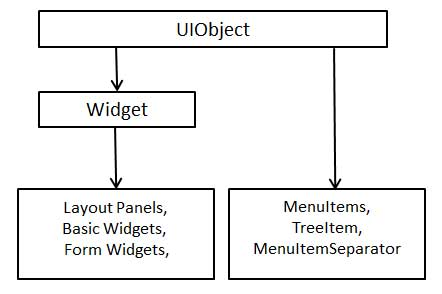
\includegraphics[width=0.7\paperwidth]{img/obr2.png}
	\end{itemize}
\end{frame}


\begin{frame}\frametitle{UI objects}
	\begin{itemize}
		\item \texttt{HTML}
        \begin{itemize}
        	\item contains arbitrary HTML code,
        	\item uses \inlinexml{<div>} element,
        	\item displayed as a block.
        \end{itemize}
		\item \texttt{Image}
        \begin{itemize}
        	\item Clipped mode -- viewport is overlaid on top of an image.
        	\item Unclipped -- whole image is visible.
        \end{itemize}
		\item \texttt{Anchor}
        \begin{itemize}
        	\item represents \inlinexml{<a>} element.
        \end{itemize}
	\end{itemize}
\begin{textblock}{15}(8.6,3.7)
    {\footnotesize Examples GwtHtml, GwtImage}
\end{textblock}
\end{frame}


\begin{frame}\frametitle{Form Widgets}
	\begin{itemize}
        \item \texttt{Label}
    	\item \texttt{Button}, \texttt{PushButton}, \texttt{ToggleButton}
    	\item \texttt{CheckBox}
    	\item \texttt{RadioButton}
    	\item \texttt{ListBox}
    	\item \texttt{SuggestBox} (autocomplete)
    	\item \texttt{TextBox}, \texttt{PasswordTextBox}
    	\item \texttt{TextArea}, \texttt{RichTextArea}
    	\item \texttt{FileUpload}
    	\item \texttt{Hidden}
	\end{itemize}
\begin{tikzpicture}[remember picture,overlay]
    \node[xshift=-0.6cm,yshift=-1.3cm] at (current page.north east){%
    
\includegraphics[width=1cm]{img/kompas}};
\end{tikzpicture}
\begin{textblock}{15}(6.1,2.1)
    {\footnotesize Examples GwtLabel, GwtButton, GwtWidgets}
\end{textblock}
\end{frame}


\begin{frame}\frametitle{Complex widgets}
	\begin{itemize}
        \item \texttt{Tree}
        \item \texttt{MenuBar}
        \item \texttt{DatePicker}
        \item \texttt{CellTree}
        \item \texttt{CellList}
        \item \texttt{CellTable}
        \item \texttt{CellBrowser}
	\end{itemize}
\begin{tikzpicture}[remember picture,overlay]
    \node[xshift=-0.6cm,yshift=-1.3cm] at (current page.north east){%
    
\includegraphics[width=1cm]{img/kompas}};
\end{tikzpicture}
\begin{textblock}{15}(-0.7,3.6)
    {\footnotesize Examples GwtComplexWidgets, GwtCellTree, GwtCellList, GwtCellTable, GwtCellBrowser}
\end{textblock}
\end{frame}


\begin{frame}[fragile]\frametitle{MenuBar}
	\lstset{language=Java, basicstyle=\footnotesize\ttfamily}
    \begin{lstlisting}
Command cmd = new Command() {
    public void execute() {
        Window.alert("You have selected a menu item!");
    }
};

MenuBar fooMenu = new MenuBar(true);  // vertical=true
fooMenu.addItem("do foo", cmd);
fooMenu.addItem("exit", cmd);

MenuBar barMenu = new MenuBar(true);
barMenu.addItem("do bar", cmd);
barMenu.addItem("exit", cmd);
...
MenuBar menu = new MenuBar();
menu.addItem("foo", fooMenu);
menu.addItem("bar", barMenu);

RootPanel.get().add(menu);
    \end{lstlisting}
\end{frame}


\begin{frame}\frametitle{Layout Panels}
	\begin{itemize}
		\item Layout panels contains other widgets.
		\item \texttt{Panel} -- abstract base class for all panels
		\item \texttt{FlowPanel} {\footnotesize (HTML flow)}
        \item \texttt{VerticalPanel}, \texttt{HorizontalPanel}
		\item \texttt{HorizontalSplitPanel}, \texttt{VerticalSplitPanel}
		\item \texttt{FlexTable} {\footnotesize (creates cells on demand)}
		\item \texttt{Grid}
		\item \texttt{DeckPanel} {\footnotesize (only one child widget visible, used by \texttt{TabPanel})}
		\item \texttt{DockPanel} {\footnotesize (similar to the \texttt{FullPageLayout} in the PrimeFaces)}
		\item \texttt{HTMLPanel}
		\item \texttt{TabPanel}
        \item \texttt{SimplePanel} {\footnotesize (contains only one widget)}
        \item \texttt{ScrollPanel}
        \item \texttt{FocusPanel}  {\footnotesize (makes its contents focusable)}
        \item \texttt{FormPanel}  {\footnotesize (has ability to catch mouse and keyboard events)}
		\item \texttt{PopupPanel}, \texttt{DialogBox}
		\item \texttt{Composite} {\footnotesize (widget that can wrap another widget, hiding the wrapped widget's methods)}
	\end{itemize}
\begin{tikzpicture}[remember picture,overlay]
    \node[xshift=-0.6cm,yshift=-1.3cm] at (current page.north east){%
    
\includegraphics[width=1cm]{img/kompas}};
\end{tikzpicture}
\begin{textblock}{15}(7.6,-0.3)
    {\footnotesize Examples GwtPanels, GwtFlowPanel}
\end{textblock}
\end{frame}


\begin{frame}[fragile]\frametitle{Event handling}
	\begin{itemize}
		\item Listener interface defined for each event.
		\item Classes wishing to react must implement given interface.
		\item All event handlers extends \texttt{EventHandler} interface.
		\item Callback argument is allways of type \texttt{Event}
        \item[]
        	\lstset{language=Java, basicstyle=\footnotesize\ttfamily}
            \begin{lstlisting}
public class MyClickHandler implements ClickHandler {
    @Override
    public void onClick(ClickEvent event) {
        Window.alert("Hello World!");
    }
}

Button button = new Button("Click Me!");
button.addClickHandler(new MyClickHandler());
            \end{lstlisting}
	\end{itemize}
\begin{textblock}{15}(10.4,2.1)
    {\footnotesize Example GwtEvents}
\end{textblock}
\end{frame}


\begin{frame}\frametitle{Custom Widgets}
	\renewcommand{\baselinestretch}{1.2}
	\begin{itemize}
		\item Three ways to create custom component
          \begin{itemize}
        	\item Extend \texttt{Composite} class -- easiest
              \begin{itemize}
            	\item Sencha GXT library
              \end{itemize}
            \item Use GWT DOM API
              \begin{itemize}
                \item complicated, use with caution
                \item Vaadin framework
              \end{itemize}
            \item Use Javascript, wrap it via JSNI (JavaScript Native Interface)
              \begin{itemize}
            	\item Smart GWT library
              \end{itemize}
          \end{itemize}
		\item Internal widgets can be still styled via CSS.
	\end{itemize}
	\renewcommand{\baselinestretch}{1}
\begin{textblock}{15}(4.5,3.3)
    {\footnotesize Examples GwtCustomWidgets, SmartUpload (Java 1.8)}
\end{textblock}
\end{frame}


\begin{frame}\frametitle{GWT UI Binder}
	\begin{itemize}
		\item GWT UI Binder is a framework designed to separate functionality and View of User Interface.
		\item Allows developers to build GWT applications as HTML pages with GWT widgets configured through them.
		\item Makes easier collaboration with UI designers who are more comfortable with XML, HTML and CSS than with Java source code.
		\item Provides a declarative way of defining user Interface.
		\item The UIBinder is similar to what JSP is to Servlets.
	\end{itemize}
\begin{tikzpicture}[remember picture,overlay]
    \node[xshift=-0.6cm,yshift=-1.3cm] at (current page.north east){%
    
\includegraphics[width=1cm]{img/oko}};
\end{tikzpicture}
\end{frame}


\begin{frame}[fragile]\frametitle{Steps for using UI binder}
	\begin{itemize}
		\item Create UI Declaration XML File (e. g. \texttt{Login.ui.xml})
		\item Use \texttt{ui:field} for Later Binding
        \item[] \makebox[\linewidth][l]{\inlinexml{<gwt:TextBox ui:field="loginBox" res:styleName="style.box" />}}
		\item Create Java counterpart of UI XML (e. g. \texttt{Login.java})
		\item Bind Java UI fields with \texttt{UiField} annotation
        \item[] {\footnotesize \texttt{@UiField}}
        \item[] {\footnotesize \texttt{TextBox loginBox;}}
        \item[] \ldots
        \item[] {\footnotesize \texttt{@UiHandler("loginBox")}}
        \item[] {\footnotesize \texttt{void handleLoginChange(ValueChangeEvent<String> event) \{}}
        \item[] {\footnotesize \verb+    ...+}
		\item Bind Java UI with UI XML with \texttt{UiTemplate} annotation
        \item[] {\footnotesize \texttt{@UiTemplate("Login.ui.xml")}}
        \item[] {\footnotesize \texttt{interface LoginUiBinder extends UiBinder<Widget, Login> \{}}
        \item[] {\footnotesize \texttt{\}}}
	\end{itemize}
\end{frame}


\begin{frame}[fragile]\frametitle{Steps for using UI binder}
	\begin{itemize}
		\item Create CSS File (e. g. \texttt{Login.css})
        \item[] \begin{footnotesize} \begin{verbatim}
.blackText {
    font-family: Arial, Sans-serif;
    color: #000000;
}
\end{verbatim} \end{footnotesize}
		\item Create Java based Resource File for CSS File (e.~g.~\texttt{LoginResources.java})
        \item[] \lstset{language=Java, basicstyle=\footnotesize\ttfamily}
                \begin{lstlisting}
public interface LoginResources extends ClientBundle {
    public interface MyCss extends CssResource {
        String blackText();
        ...
\end{lstlisting}
		\item Attach CSS resource in Java UI Code file
        \item[] \lstset{language=Java, basicstyle=\footnotesize\ttfamily}
            \begin{lstlisting}
@UiField(provided = true)
final LoginResources res;

public Login() {  // constructor
    this.res = GWT.create(LoginResources.class);
    res.style().ensureInjected();
        \end{lstlisting}
	\end{itemize}
\begin{tikzpicture}[remember picture,overlay]
    \node[xshift=-0.6cm,yshift=-1.3cm] at (current page.north east){%
    
\includegraphics[width=1cm]{img/naradi}};
\end{tikzpicture}
\begin{textblock}{15}(11.2,-0.3)
    {\footnotesize Example GwtUI}
\end{textblock}
\end{frame}


\begin{frame}\frametitle{GWT RPC}
	\begin{itemize}
		\item RPC (Remote Procedure Call) is the mechanism used by GWT which allows the client code to directly execute the server side methods.
		\item GWT RPC is servlet based.
		\item GWT RPC is asynchronous and client is never blocked during the communication.
		\item Using GWT RPC Java objects can be sent directly between the client and the server.
		\item Server-side servlet is termed as service.
		\item Remote procedure call which is calling methods of server side servlets from client side code is referred to as invoking a service.
	\end{itemize}
\begin{tikzpicture}[remember picture,overlay]
    \node[xshift=-0.6cm,yshift=-1.3cm] at (current page.north east){%
    
\includegraphics[width=1cm]{img/pozor}};
\end{tikzpicture}
\end{frame}


\begin{frame}\frametitle{GWT RPC Components}
	\begin{itemize}
		\item A remote service (server-side servlet) runs on the server.
		\item Client code, which is invoking the service.
		\item Java data objects which will be passed between client and server.
        \medskip
		\item GWT client and server both serialize and deserialize the data automatically so developers are not required to serialize/deserialize the objects and data objects can travel over HTTP.
	\end{itemize}
\begin{tikzpicture}[remember picture,overlay]
    \node[xshift=-0.6cm,yshift=-1.3cm] at (current page.north east){%
    
\includegraphics[width=1cm]{img/oko}};
\end{tikzpicture}
\end{frame}


\begin{frame}[fragile]\frametitle{Communication with the Server}
	\begin{itemize}
		\item HTTP Client
          \begin{itemize}
        	\item ``standard'' AJAX
            \item HTTP module
              \begin{itemize}
            	\item \texttt{<inherits name="com.google.gwt.http.HTTP" />}
              \end{itemize}
          \end{itemize}
        \medskip
        \item[]
        	\lstset{language=Java, basicstyle=\footnotesize\ttfamily}
            \begin{lstlisting}
String url = "http://www.myserver.com/getData?type=3";
RequestBuilder builder = new RequestBuilder(
    RequestBuilder.GET, URL.encode(url));

Request request = builder.sendRequest(null, 
    new RequestCallback() {
  public void onError(Request request, 
                      Throwable exception) {
      //  (timeout, SOP violation, etc.)     
  }
  public void onResponseReceived(Request request, 
                                 Response response) {
    if (200 == response.getStatusCode()) {
      // Process the response in response.getText()
    } else {
      // Handle the error in response.getStatusText()
  }
});     
            \end{lstlisting}
	\end{itemize}
\end{frame}


\begin{frame}[t]\frametitle{GWT RPC workflow}
\begin{columns}
    \column{\dimexpr\paperwidth-20pt}
    \begin{itemize}
		\item Java specific protocol
          \begin{itemize}
        	\item GWT’s ``serializable'' is slightly different than standard Java Serialization 
          \end{itemize}
	\end{itemize}
    \centering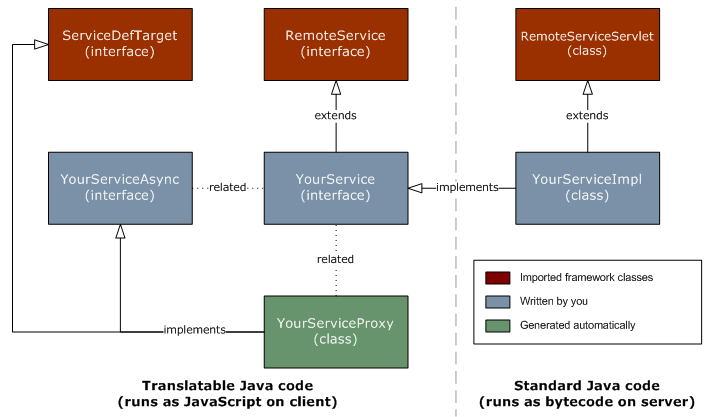
\includegraphics[width=0.95\paperwidth]{img/obr3.png}
\end{columns}
\begin{tikzpicture}[remember picture,overlay]
    \node[xshift=-0.6cm,yshift=-1.3cm] at (current page.north east){%
    
\includegraphics[width=0.9cm]{img/lupa}};
\end{tikzpicture}
\end{frame}


\begin{frame}[fragile]\frametitle{GWT RPC -- step 1}
	\begin{itemize}
		\item Create serializable model class.
        \medskip
        \item[]
        	\lstset{language=Java, basicstyle=\footnotesize\ttfamily}
            \begin{lstlisting}
public class Message implements Serializable {
    ...
    private String message;
    public Message(){};
    public void setMessage(String message){
        this.message = message;
    }
    ...
}
            \end{lstlisting}
	\end{itemize}
\begin{tikzpicture}[remember picture,overlay]
    \node[xshift=-0.6cm,yshift=-1.3cm] at (current page.north east){%
    
\includegraphics[width=1cm]{img/lupa}};
\end{tikzpicture}
\end{frame}




\begin{frame}[fragile]\frametitle{GWT RPC -- step 2}
	\begin{itemize}
		\item Create a Service Interface
          \begin{itemize}
        	\item Define an interface for service on the client side that extends \texttt{RemoteService} listing all service methods.
        	\item Use annotation \texttt{@RemoteServiceRelativePath} to map the service with a default path of remote servlet relative to~the module base URL.
          \end{itemize}
        \medskip
        \item[]
        	\lstset{language=Java, basicstyle=\footnotesize\ttfamily}
			\begin{lstlisting}
@RemoteServiceRelativePath("message")
public interface MessageService extends RemoteService {
    Message getMessage(String input);
}
			\end{lstlisting}
	\end{itemize}
\begin{tikzpicture}[remember picture,overlay]
    \node[xshift=-0.6cm,yshift=-1.3cm] at (current page.north east){%
    
\includegraphics[width=1cm]{img/lupa}};
\end{tikzpicture}
\end{frame}


\begin{frame}[fragile]\frametitle{GWT RPC -- step 3}
	\begin{itemize}
		\item {Create an Async Service Interface}
          \begin{itemize}
			\item Define an asynchronous interface to the service on the client side which will be used in the GWT client code.
            \item Async Service Interface can be generated automatically -- in the Maven \texttt{<goal>generateAsync</goal>}
          \end{itemize}
		\item[]
        	\lstset{language=Java, basicstyle=\footnotesize\ttfamily}
            \begin{lstlisting}
public interface MessageServiceAsync {
    void getMessage(String input, 
                    AsyncCallback<Message> callback);
}
            \end{lstlisting}
	\end{itemize}
\begin{tikzpicture}[remember picture,overlay]
    \node[xshift=-0.6cm,yshift=-1.3cm] at (current page.north east){%
    
\includegraphics[width=1cm]{img/lupa}};
\end{tikzpicture}
\end{frame}


\begin{frame}[fragile]\frametitle{GWT RPC -- step 4}
	\begin{itemize}
		\item Create a Service Implementation Servlet class.
		\item Implement the interface at the server side and that class should extend \texttt{RemoteServiceServlet} class.
        \item[]
        	\lstset{language=Java, basicstyle=\footnotesize\ttfamily}
			\begin{lstlisting}
public class MessageServiceImpl 
        extends RemoteServiceServlet
        implements MessageService {
    ...
    public Message getMessage(String input){
        String messageString = "Hello " + input + "!";
        Message message = new Message();
        message.setMessage(messageString);
        return message;
    }
}
			\end{lstlisting}
	\end{itemize}
\begin{tikzpicture}[remember picture,overlay]
    \node[xshift=-0.6cm,yshift=-1.3cm] at (current page.north east){%
    
\includegraphics[width=1cm]{img/lupa}};
\end{tikzpicture}
\end{frame}


\begin{frame}[fragile]\frametitle{GWT RPC -- step 5}
	\begin{itemize}
		\item Update \texttt{web.xml} to include the servlet declaration.
        \medskip
		\item[]
        	\lstset{language=XML, basicstyle=\footnotesize\ttfamily}
			\begin{lstlisting}
<web-app>
    ...
    <servlet>
        <servlet-name>messageServiceImpl</servlet-name>
        <servlet-class>
          com.tutorialspoint.server.MessageServiceImpl
        </servlet-class>
    </servlet>
    <servlet-mapping>
        <servlet-name>messageServiceImpl</servlet-name>
        <url-pattern>/helloworld/message</url-pattern>
    </servlet-mapping>
</web-app>
			\end{lstlisting}
	\end{itemize}
\begin{tikzpicture}[remember picture,overlay]
    \node[xshift=-0.6cm,yshift=-1.3cm] at (current page.north east){%
    
\includegraphics[width=1cm]{img/lupa}};
\end{tikzpicture}
\end{frame}


\begin{frame}[fragile]\frametitle{GWT RPC -- step 6}
  \begin{itemize}
	\item Make the remote procedure call in the application code.
      \begin{itemize}
		\item Create the service proxy class.
          \begin{itemize}
        	\item
            	\lstset{basicstyle=\footnotesize\ttfamily}
            	\inlinejava{MessageServiceAsync messageService = GWT.create(MessageService.class);}
          \end{itemize}
        \item Create the \texttt{AsyncCallback} handler to handle RPC callback in which server returns the Message back to the client.
      \end{itemize}
  \end{itemize}
\begin{tikzpicture}[remember picture,overlay]
    \node[xshift=-0.6cm,yshift=-1.3cm] at (current page.north east){%
    
\includegraphics[width=1cm]{img/lupa}};
\end{tikzpicture}
\end{frame}


\begin{frame}[fragile]\frametitle{GWT RPC -- finished}
	\lstset{language=Java, basicstyle=\footnotesize\ttfamily}
    \begin{lstlisting}
class MessageCallBack implements AsyncCallback<Message> {
  @Override
  public void onFailure(Throwable caught){
    Window.alert("Unable to obtain server response: " + caught.getMessage());
  }
  @Override
  public void onSuccess(Message result){
    Window.alert(result.getMessage());
  }
}
public class HelloWorld implements EntryPoint {
  private MessageServiceAsync messageService = GWT.create( ...
  ...
  public void onModuleLoad(){
  ...
    buttonMessage.addClickHandler(new ClickHandler(){
      @Override
      public void onClick(ClickEvent event){
        messageService.getMessage(txtName.getValue(),
          new MessageCallBack());
      }});
  ...
  }
}
    \end{lstlisting}
\begin{textblock}{15}(10.8,-1.0)
    {\footnotesize Example GwtRpc}
\end{textblock}
\end{frame}


\begin{frame}\frametitle{GWT Internationalization}
	\begin{itemize}
		\item Three ways to internationalize GWT Application
          \begin{itemize}
        	\item Static String Internationalization\\
              \begin{itemize}
            	\item Little overhead in runtime
                \item Constants and parametrized strings
              \end{itemize}
            \item Dynamic String Internationalization\\
              \begin{itemize}
            	\item More flexible
                \item For integrating with existing ``localized'' server
              \end{itemize}
            \item Localizable interface\\
              \begin{itemize}
            	\item The most powerful
                \item Custom localizable types
              \end{itemize}
          \end{itemize}
	\end{itemize}
\begin{tikzpicture}[remember picture,overlay]
    \node[xshift=-0.6cm,yshift=-1.3cm] at (current page.north east){%
    
\includegraphics[width=1cm]{img/oko}};
\end{tikzpicture}
\end{frame}


\begin{frame}[fragile]\frametitle{Internationalization process}
Static String Internationalization
	\begin{itemize}
		\item Create properties files
          \begin{itemize}
        	\item \texttt{HelloWorld.properties} {\footnotesize(default language)}
            \itmspace{.5em} {\texttt{HelloWorld\_cs.properties} {\footnotesize(czech version)}}
          \end{itemize}
		\item Add i18n module to the Module Descriptor XML File
        \item[]
            \lstset{language=XML, basicstyle=\ttfamily}
            \begin{lstlisting}
<extend-property name="locale" values="cs"/>
            \end{lstlisting}
        \item Create interface equivalent to the properties file.
        \item Use \texttt{Message} interface in the UI component.
	\end{itemize}
\begin{tikzpicture}[remember picture,overlay]
    \node[xshift=-0.6cm,yshift=-1.3cm] at (current page.north east){%
    
\includegraphics[width=1cm]{img/oko}};
\end{tikzpicture}
\end{frame}


\begin{frame}[fragile]\frametitle{Internationalization properties}
	\begin{itemize}
		\item \texttt{HelloWorld.properties}
		\item[]
        	\footnotesize
        	\begin{verbatim}
enterName=Enter your name
clickMe=ClickMe
applicationTitle=Application Internationalization Demonstration
greeting=Hello{0}
        	\end{verbatim}
            \normalsize
		\item \texttt{HelloWorld\_cs.properties} 
          \begin{itemize}
            \item \emph{Unicode !!!}
          \end{itemize}
       	\item[]
        	\footnotesize
        	\begin{verbatim}
enterName=Napi\u0161te sv\u0117 jm\u0117no
clickMe=Klikn\u011Bte sem
applicationTitle=Demonstrace internacionalizace aplikace
greeting=Ahoj{0}
        	\end{verbatim}
            \normalsize
	\end{itemize}
\end{frame}


\begin{frame}[fragile]\frametitle{Internationalization usage}
	\begin{itemize}
		\item Translated application available at \url{http://127.0.0.1:8888/HelloWorld.html?gwt.codesvr=127.0.0.1:9997&locale=cs}
        \medskip
        \item[]
        	\lstset{language=Java, basicstyle=\footnotesize\ttfamily}
            \begin{lstlisting}
public interface HelloWorldMessages extends Messages{
    @DefaultMessage("Enter your name")
    String enterName();
    @DefaultMessage("Click Me")
    String clickMe();
    @DefaultMessage("Application Internalization Demonstration")
    String applicationTitle();
    @DefaultMessage("Hello {0}")
    String greeting(String name);
}
            \end{lstlisting}
	\end{itemize}
\begin{tikzpicture}[remember picture,overlay]
    \node[xshift=-0.6cm,yshift=-1.3cm] at (current page.north east){%
    
\includegraphics[width=1cm]{img/naradi}};
\end{tikzpicture}
\begin{textblock}{15}(8.3,1.5)
    {\footnotesize Example GwtInternationalization}
\end{textblock}
\end{frame}


\begin{frame}[fragile]\frametitle{Bookmarkable History}
	\begin{itemize}
		\item ``AJAX'' applications breaks browser ``back'' button.
        \item GWT History mechanism
          \begin{itemize}
            \item History tokens
              \begin{itemize}
            	\item \verb'http://www.example.com/helloworld/Hello.html#page1'
              \end{itemize}
            \item History
              \begin{itemize}
                \item get the current URL fragment (\texttt{page1})
                \item[] \inlinejava{String getToken()}\\[0.3em]
                \item add new history token to the history stack
                \item[] \inlinejava{newItem(String token)}\\[0.3em]
                \item Event of history change
                \item[] \inlinejava{ValueChangeEvent}   
              \end{itemize}
            \item Link to another state of the running application. 
              \begin{itemize}
                \item When clicked, it will create a new history frame without reloading the page.
              \end{itemize}
            \item[] \inlinejava{Hyperlink(String text, String token)}\\[0.3em]
            \item Reconstruct all the application state from the token.
          \end{itemize}
	\end{itemize}
\end{frame}


\begin{frame}[fragile]\frametitle{History Management Workflow}
	\begin{itemize}
		\item Enable History support
        \item[] 
        	\lstset{language=XML, basicstyle=\ttfamily}
        	\begin{lstlisting}
<iframe	src = "javascript:''" 
        id = "__gwt_historyFrame" 
        style = "width:0;height:0;border:0">
</iframe>
        	\end{lstlisting}
		\item Add token to the history
        \item[] 
            \lstset{language=Java, basicstyle=\footnotesize\ttfamily}
            \begin{lstlisting}
index = 0;
History.newItem("pageIndex" + index);
			\end{lstlisting}
		\item Retrieve token from the history
		\item[]
        	\lstset{language=Java, basicstyle=\footnotesize\ttfamily}
            \begin{lstlisting}
History.addValueChangeHandler(
    new ValueChangeHandler<String>(){
  @Override
  public void onValueChange(ValueChangeEvent<String>event){
    String historyToken = event.getValue();
    ...
            \end{lstlisting}
	\end{itemize}
\begin{tikzpicture}[remember picture,overlay]
    \node[xshift=-0.6cm,yshift=-1.3cm] at (current page.north east){%
    
\includegraphics[width=1cm]{img/naradi}};
\end{tikzpicture}
\begin{textblock}{15}(10.4,-0.2)
    {\footnotesize Example GwtHistory}
\end{textblock}
\end{frame}


\begin{frame}[fragile]\frametitle{Delayed logic}
	\begin{itemize}
		\item \texttt{Timer}
          \begin{itemize}
        	\item \inlinejava{schedule(int delayMillis)}
            \item \inlinejava{scheduleRepeating(int periodMillis)}
          \end{itemize}
        \item[]
            \lstset{language=Java, basicstyle=\footnotesize\ttfamily}
            \begin{lstlisting}
Timer timer = new Timer() {
    public void run() {
        Window.alert ("Timer expired!");
    }
};
timer.schedule(2000);
            \end{lstlisting}
		\item \texttt{RepeatingCommand}
        \begin{itemize}
       		\item
            	\lstset{language=Java, basicstyle=\footnotesize\ttfamily}
                \begin{lstlisting}
Scheduler scheduler = Scheduler.get();
scheduler.scheduleIncremental(repCmd, delayMs);
                \end{lstlisting}
                \vspace{-.5em}
                \begin{itemize}
                    \item The next invocation of the command will be scheduled for \texttt{delayMs} milliseconds after the last invocation completes.
                \end{itemize}
            \item \inlinejava{Scheduler.RepeatingCommand}
              \begin{itemize}
                \item command to be executed
            	\item for breaking long running tasks into chunks
				\item \verb+boolean execute()  // Returns true if the+
                \item[] \verb+                   // RepeatingCommand should be +
                \item[] \verb+                   // invoked again.+
              \end{itemize}   
		\end{itemize}   
	\end{itemize}
\end{frame}


\begin{frame}[fragile]\frametitle{Drawing in GWT}
	\renewcommand{\baselinestretch}{1.2}
	\begin{itemize}
		\item \texttt{Canvas}
          \begin{itemize}
            \item drawing area
            \item \texttt{getContext2d()}
          \end{itemize}
		\item \texttt{Context2D}
          \begin{itemize}
            \item no \texttt{onDraw} as in Swing
            \item we are drawing directly (e.g. on button click)
        	\ttfamily
        	\item Arc
        	\item DrawImage
        	\item FillRect
        	\item FillText
        	\item StrokeRect
        	\item StrokeText
        	\item Scale
        	\item Rotate
        	\item Translate
          \end{itemize}
	\end{itemize}
    \renewcommand{\baselinestretch}{1}
\begin{tikzpicture}[remember picture,overlay]
    \node[xshift=-0.6cm,yshift=-1.3cm] at (current page.north east){%
    
\includegraphics[width=1cm]{img/kompas}};
\end{tikzpicture}
\begin{textblock}{15}(11.6,0.1)
    {\footnotesize Example Kufr}
\end{textblock}
\end{frame}


\begin{frame}[fragile]\frametitle{JavaScript Native Interface (JSNI)}
	\begin{itemize}
		\item JSNI allows Java and JavaScript interaction.
		\item JSNI methods are declared \texttt{native}.
		\item Special syntax
          \begin{itemize}
        	\item Begins with \verb'/*-{'
            \item End with \verb'}-*/;'
          \end{itemize}
		\item JSNI syntax is \emph{Java-to-JavaScript} compiler directive.
		\item Special variables
          \begin{itemize}
        	\item \verb|$doc| -- refers to document
        	\item \verb|$wnd| -- refers to browser’s window
          \end{itemize}
	\end{itemize}
\begin{tikzpicture}[remember picture,overlay]
    \node[xshift=-0.6cm,yshift=-1.3cm] at (current page.north east){%
    
\includegraphics[width=1cm]{img/pozor}};
\end{tikzpicture}
\end{frame}


\begin{frame}[fragile]\frametitle{JSNI examples}
	\begin{itemize}
    	\item Parameter passing is simple
		\item[]
        	\lstset{language=Java, basicstyle=\footnotesize\ttfamily}
			\begin{lstlisting}
public static native void alert(String msg) /*-{
    $wnd.alert(msg);
}-*/;
public static native int inv(int num) /*-{
    return -num;
}-*/
public static void printInv(int num){
    System.out.println(inv(num));
}
			\end{lstlisting}
		\item Type mismatch
			\lstset{language=Java, basicstyle=\footnotesize\ttfamily}
			\begin{lstlisting}
public static native int badExample() /*-{
    return "Not A Number";
}-*/;
public void onClick () {
    try {
        int myValue = badExample();
        GWT.log("Got value " + myValue, null);
    } catch (Exception e) {
        GWT.log("JSNI method badExample() threw an exception:", e);
    }
}
			\end{lstlisting}
	\end{itemize}
\end{frame}



\begin{frame}[fragile]\frametitle{\normalsize{Accessing Java methods and fields from JavaScript}}
	\begin{itemize}
		\item It is possible to manipulate Java objects in JavaScript code.
		\item Invoking Java methods from JavaScript
        \begin{itemize}
        	\footnotesize
        	\item[] \verb'[instance-expr.]@Class-name::method-name(param-signature)'
            \verb'(arguments)'\\[1em]
            \item \textbf{instance-expr} -- necessary when calling instance method (must be absent when calling static one) (mostly \texttt{this})
            \item \textbf{Class-name} -- fully qualified, contains path in package
            \item \textbf{param-signature} -- uses JNI type signatures
            \item \textbf{arguments} -- passed variables
            \normalsize
        \end{itemize}
     	\item JNI (Java Native Interface)
     	\begin{itemize}
        	\item \texttt{D} -- double
        	\item \texttt{I} -- int
        	\item \texttt{C} -- char
        	\item \texttt{L} -- follows fully qualified name (\texttt{Ljava/lang/String;})
        	\item \ldots
     	\end{itemize}
	\end{itemize}
\begin{tikzpicture}[remember picture,overlay]
    \node[xshift=-0.6cm,yshift=-1.3cm] at (current page.north east){%
    
\includegraphics[width=1cm]{img/lupa}};
\end{tikzpicture}
\end{frame}


\begin{frame}[fragile]\frametitle{JSNI calls}
	\begin{itemize}
		\item Constructor
          \begin{itemize}
        	\item \inlinejava{new TopLevel()} becomes \inlinejava{@pkg.TopLevel::new()()}
            \itmspace{0.5em} {\inlinejava{new StaticInner()} becomes \inlinejava{@pkg.TopLevel.StaticInner::new()()}}
            \item \inlinejava{someTopLevelInstance.new InstanceInner(123)} becomes \inlinejava{@pkg.TopLevel.InstanceInner::new(Lpkg/TopLevel;I)}
            \item[] \inlinejava{(someTopLevelInstance, 123)}
            \begin{itemize}
            	\item Enclosing instance is the first parameter.
            \end{itemize}
          \end{itemize}
        \smallskip
        \item Accessing Java fields from JavaScript
          \begin{itemize}
        	\item \verb'[instance-expr.]@class-name::field-name'
          \end{itemize}
	\end{itemize}
\end{frame}


\begin{frame}[fragile]\frametitle{JSNI calls}
	\begin{itemize}
		\item Calling Java methods from handwritten JavaScript
        \item[]
        	\lstset{language=Java, basicstyle=\footnotesize\ttfamily}
            \begin{lstlisting}
package mypackage;

public MyUtilityClass
{
  public static int computeLoanInterest(int amt, 
                                        float interestRate,
                                        int term) { ... }
  public static native void exportStaticMethod() /*-{
    $wnd.computeLoanInterest =
      $entry(@mypackage.MyUtilityClass::computeLoanInterest(IFI));
  }-*/;
}
            \end{lstlisting}
        \item {\small Notice that the reference to the exported method has been wrapped in a call to the \texttt{\$entry} function. This implicitly-defined function ensures that the Java-derived method is executed with the uncaught exception handler installed and pumps a number of other utility services. The \texttt{\$entry} function is reentrant-safe and should be used anywhere that GWT-derived JavaScript may be called into from a non-GWT context.}
	\end{itemize}
\end{frame}


\begin{frame}[fragile]\frametitle{Passing Java values into JavaScript}
	\begin{footnotesize}
    	\renewcommand{\arraystretch}{1.7}
        \rowcolors{1}{blue!10}{white}
        \begin{tabular}{p{4.5cm} p{5.5cm}}
        \rowcolor{blue!20}
        \vspace{.05pt}
        \textbf{Outcoming Java type} & \vspace{.05pt} \textbf{How it appears to JavaScript code}\\[.05pt]
        \scriptsize
        
		String & \texttt{var s = \color{red}”my string”}\\
        boolean & \texttt{var b = true}\\
        long & disallowed to pass into JavaScript (in Java it can be emulated)\\
        numeric primitives & \texttt{var x = 10}\\
        JavaScriptObject & JavaScriptObject that must have originated from JavaScript code, typically as the return value of some other JSNI method\\
        Java Array & can only be passed back to java code\\
        any other object & accessible via special syntax (with \texttt{L})
        \normalsize
        \end{tabular}
        \renewcommand{\arraystretch}{1}
	\end{footnotesize}
\end{frame}

\begin{frame}[fragile]\frametitle{Passing JavaScript values into Java code}
	\begin{footnotesize}
    	\renewcommand{\arraystretch}{1.7}
        \rowcolors{1}{blue!10}{white}
        \begin{tabular}{p{5cm} p{5cm}}
        \rowcolor{blue!20}
        \vspace{.05pt}
        \textbf{Incoming Java type} & \vspace{.05pt} \textbf{What must be passed}\\[.05pt]
        \scriptsize
        String & JavaScript string, as \texttt{return \color{red}"abc"\color{black};}\\
        boolean & JavaScript boolean value, as in \texttt{return true;}\\
        long & disallowed\\
        numeric primitives & JavaScript numeric value, as in \texttt{return 10;}\\
        JavaScriptObject & some native JavaScript object, as in \texttt{return document.createElement(\color{red}"div"\color{black})}\\
        any other object (including arrays) & must originate from Java code
        \normalsize
        \end{tabular}
        \renewcommand{\arraystretch}{1}
	\end{footnotesize}
\end{frame}


\begin{frame}\frametitle{JSNI exceptions}
	\begin{itemize}
		\item An exception can be thrown during the execution of either normal Java code or the JavaScript code within a JSNI method.
		\item One can catch \texttt{JavaScriptException}
          \begin{itemize}
        	\item contains only class name and description.
          \end{itemize}
		\item Exceptions originating from Java code retain its identity.
          \begin{itemize}
        	\item When Java calls JavaScript and JavaScript calls Java, where an exception occurs
          \end{itemize}
	\end{itemize}
\end{frame}


\begin{frame}[fragile]\frametitle{Further examples (1/2)}
	\lstset{language=Java, basicstyle=\footnotesize\ttfamily}
	\begin{lstlisting}
public class JSNIExample {
  String myInstanceField;
  static int myStaticField;
  void instanceFoo(String s) {
    // use s
  }
  static void staticFoo(String s) {
    // use s
  }
	\end{lstlisting}
\end{frame}


\begin{frame}[fragile]\frametitle{Further examples (2/2)}
	\lstset{language=Java, basicstyle=\footnotesize\ttfamily}
	\begin{lstlisting}
  
  public native void bar(JSNIExample x, String s) /*-{
    // Call instance method instanceFoo() on this
    this.@com.google.gwt.examples.JSNIExample::instanceFoo
        (Ljava/lang/String;)(s);
    // Call instance method instanceFoo() on x
    x.@com.google.gwt.examples.JSNIExample::instanceFoo
        (Ljava/lang/String;)(s);
    // Call static method staticFoo()
    @com.google.gwt.examples.JSNIExample::staticFoo
        (Ljava/lang/String;)(s);
    // Read instance field on this
    var val = this.@com.google.gwt.examples.JSNIExample::myInstanceField;
    // Write instance field on x
    x.@com.google.gwt.examples.JSNIExample::myInstanceField = val + " and stuff";
    // Read static field (no qualifier)
    @com.google.gwt.examples.JSNIExample::myStaticField = val + " and stuff";
  }-*/;
}
	\end{lstlisting}
\end{frame}


\begin{frame}\frametitle{Resources}
	\begin{itemize}
        \item \url{http://www.gwtproject.org/}
        \item \url{http://www.gwtproject.org/javadoc/latest/}
        \item \url{http://samples.gwtproject.org/samples/Showcase/Showcase.html}
        \medskip
        \item \url{http://www.gwtproject.org/doc/latest/tutorial/}
        \item \url{http://www.gwtproject.org/doc/latest/DevGuide.html}
        \item \url{https://gwt-maven-plugin.github.io/gwt-maven-plugin/}
		\item \url{http://www.tutorialspoint.com/gwt/}
		\item \url{https://tbroyer.github.io/gwt-maven-plugin/}
		\item \url{https://medium.com/star-gazers/gwt-boot-starters-bootstrap-a-simple-gwt-web-app-568559556a2c}
	\end{itemize}
\end{frame}



\bluepage{Thank you for your attention!}



\end{document}
